\documentclass{article}
\usepackage[T1]{fontenc}
\usepackage{lmodern}
\usepackage{graphicx}
\usepackage{amsmath,amssymb}
\usepackage[a4paper,margin=2cm]{geometry}
\usepackage[absolute,overlay]{textpos}
\setlength{\TPHorizModule}{1mm}
\setlength{\TPVertModule}{1mm}
\usepackage[indonesian]{babel}
\usepackage{hyperref}
\setlength{\emergencystretch}{2em}
% unit: Halaman 22

\begin{document}

% === Halaman 22 (llm) ===

Demo DH online: https://asecuritysite.com/encryption/diffie

\section*{Diffie-Hellman Example}

\vspace{201.96mm}

[Encryption Home][Home]

Diffie-Hellman is a standard method of Alice and Bob being able to communicate, and end up with the same secret encryption key. It is used in many applications, and uses two numbers (G and N) for the first part of the calculation (of which N must be a prime number):

[Related Lecture] [Tutorial] [Software Tutorial] [Software Lecture] [Theory] [Blog] [Picking G value]

G: 1601 \\
N: 4789

\vspace{10mm}

Next Bob and Alice will generate two random numbers (X and Y), calculate an X value and a Y value, respectively:

\begin{tabular}{ll} 
Bob's X Value & 20 \\
Bob's random value & \\
Bob's A value & 2716 \\
$A = G^{x} \pmod{N}$ & \\
\end{tabular} 
\begin{tabular}{ll} 
Alice's Y value & 4 \\
Alice's random value & \\
Alice's B value & 1302 \\
$B = G^{y} \pmod{N}$ & \\
\end{tabular}

% deskripsi: Tampilan antarmuka web simulasi Diffie-Hellman yang menunjukkan input nilai G, N serta perhitungan nilai A dan B untuk Bob dan Alice.
% bbox normalisasi: [0.0400, 0.2100, 0.8500, 0.8900]
\begin{textblock*}{170.10mm}(8.40mm,62.37mm)
\noindent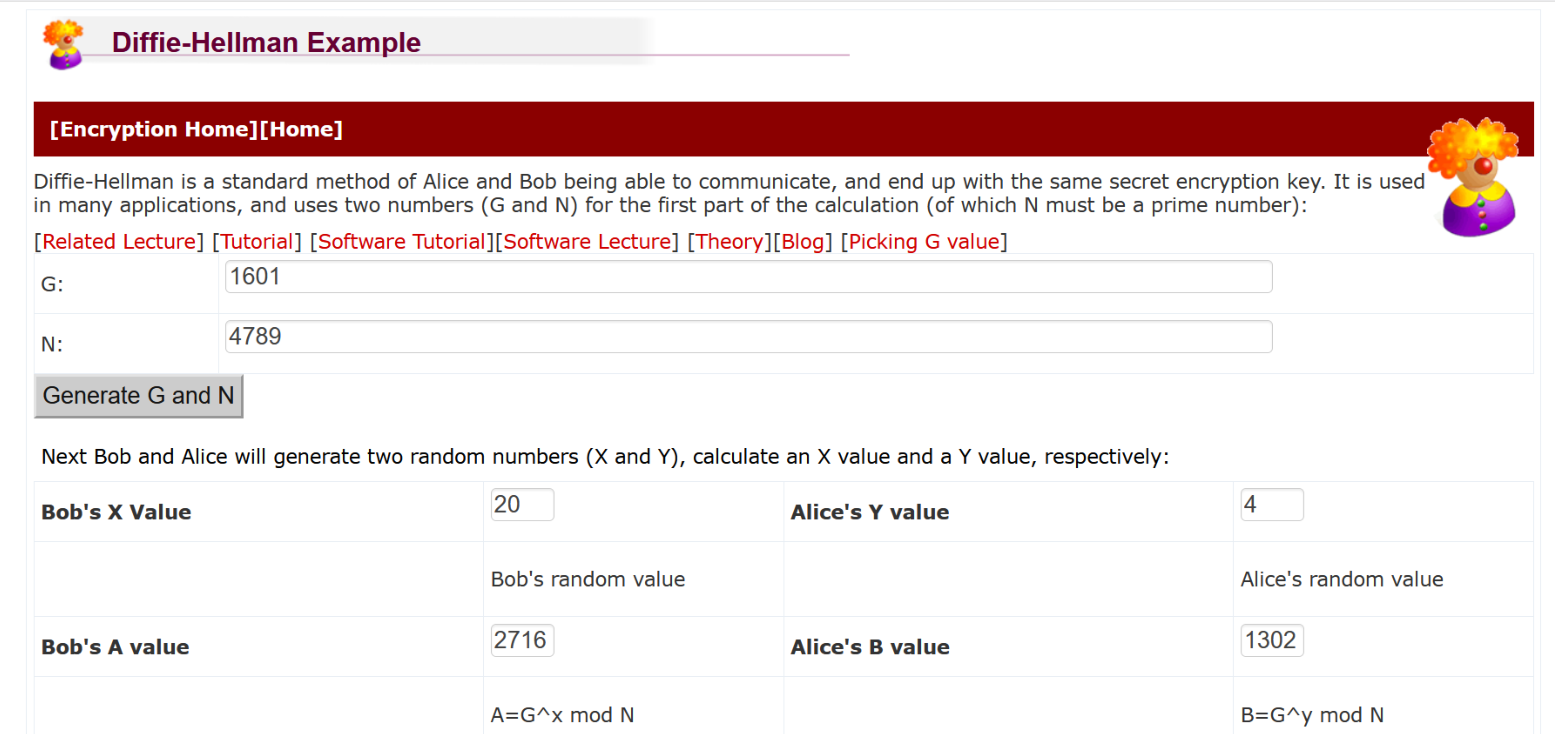
\includegraphics[width=170.10mm,height=201.96mm]{../../images/llm/page_022_img_01.png}%
\end{textblock*}

\end{document}
